\documentclass[11pt]{article}
\usepackage[left=1in,right=1in,top=0.75in,bottom=0.75in]{geometry}
\usepackage{amsmath}
\usepackage{graphicx}
\usepackage{float}
\usepackage[hidelinks]{hyperref}
\usepackage{microtype}

\begin{document}

Hello professor, here is a higher level overview of the projects I have been working on since being admitted to your group this recent January. This report also indicates how Jacopo and I have visualized the subsequent work-load/paper trajectories, and the preliminary results of each so far.

As a brief note on workload, last semester I took two courses in addition to your research credit, while being enrolled as a teacher assistant for Physics 104 with the responsibility of discussions 4x/week and labs 2x/week along with substituting for other TAs. I am enrolled in a course this summer.
or workload, there were numerous nights that I slept at the Physics office to save commute time (although now I live only 4 blocks away from the MSE building).

Here is what I have worked on and the road-map:

\subsubsection*{Paper I: ADAPT-VQE Ground State}
My algorithm ranks operators ($A$) by energy per cost $\Delta E / K$ within a position $p$ of the current ansatz circuit $U(\theta)$. So I write the pair as:
\[
r=(A,p) \mapsto e^{i\alpha A} \mapsto U(\theta)| \phi_{\rm ref} \rangle=|\psi\rangle.
\]
Novelty:

- Shortlisting of records to get higher order energy modeling with number of quantum measurements less than scoring/modeling the full operator pool.

- Scoring operators per unit hardware cost.

- Insertion was recently introduced by GEO-ADAPT this May, but they found little benefit in their algorithm, whereas mine establishes more benefit and also the activation of insertion-scoring occurs during energy-gradient plateaus which likewise saves costs.

- Operator pool definition for Hubbard--Holstein model with high physical response channel relevance.

- Energy model for adding multiple operators at once, energy model for deleting an operator from $U(\theta)$, and the first application of Lowrerre beam search to ADAPT-VQE.

- Gram matrix which allows for Trust-region based modeling, and allows for the whitening of coordinates (produces orthonormal basis on retained non-null tangent support) which helps inner optimization procedures.


\subsubsection*{Paper II: Time Dynamics of Hubbard--Holstein}
This project time-evolves a Paper-I ground-state ansatz with the McLachlan variational principle. The main additions are:

- State-space numerical stabilization through regularized linear solves and local time-step subdivision.

- Cost-weighted addition and deletion of ansatz generators during propagation. Adaptive addition already exists in the literature; to the best of my current search, online generator deletion during McLachlan dynamics does not.

- Quantum simulation of driven Hubbard--Holstein energy, site occupations, and doublon dynamics.

Figure~\ref{fig:paper-ii-results} uses the same redundant 118-parameter ansatz, Gaussian drive ($A=0.8$), and time grid through $t=5$ for all three comparisons. Reductions relative to fixed McLachlan are:

\begin{center}
\small
\begin{tabular}{lrrrr}
\hline
Method & \shortstack{Energy-error\\reduction} & \shortstack{Doublon-error\\reduction} & \shortstack{Parameter\\reduction} & \shortstack{$N_{2q}$\\reduction} \\
\hline
Stabilization & $14.5\%$ & $47.9\%$ & $0\%$ & $0\%$ \\
Stabilization + pruning & $37.0\%$ & $70.3\%$ & $24.6\%$ & $33.0\%$ \\
\hline
\end{tabular}
\end{center}

\begin{figure}[H]
    \centering
    \small\textbf{Legend:} blue: McLachlan propagation; orange and green: exact references; pale bands: numerical stabilization; red diamonds: accepted deletions.
    \par\medskip
    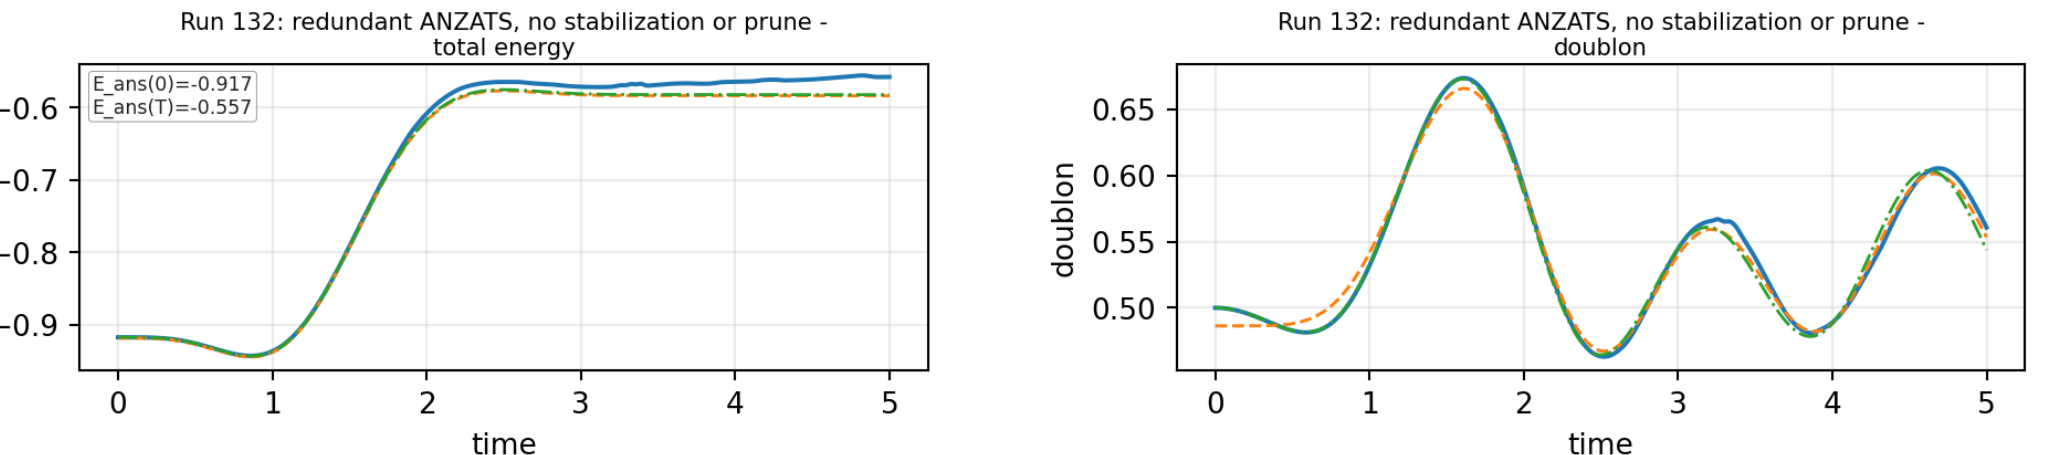
\includegraphics[width=0.80\linewidth]{advisor_project_overview_assets/results_pdf_crops/run132_fixed_energy_doublon.png}
    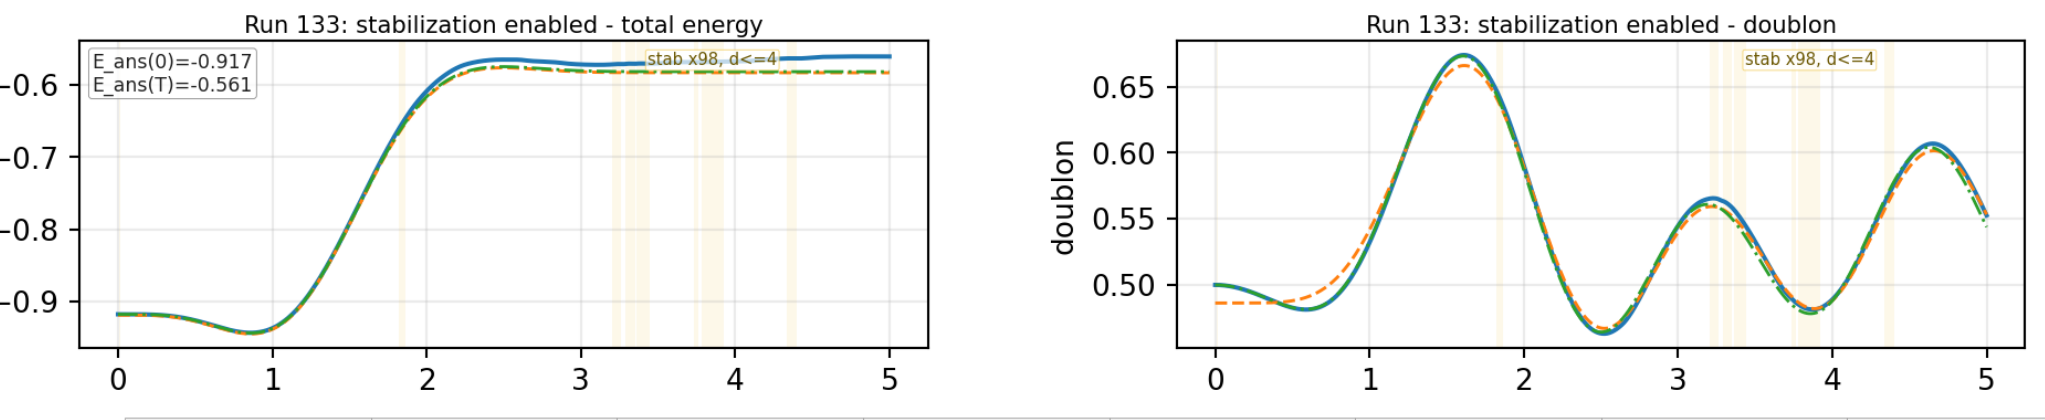
\includegraphics[width=0.80\linewidth]{advisor_project_overview_assets/results_pdf_crops/run133_stabilization_energy_doublon.png}
    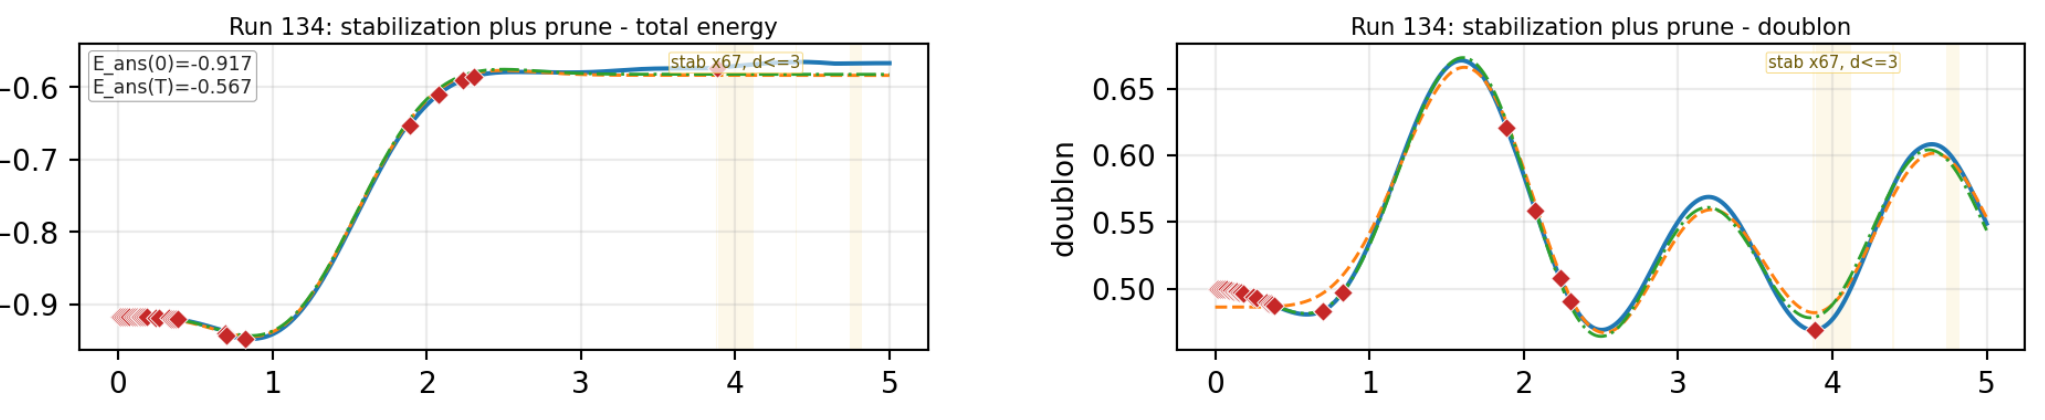
\includegraphics[width=0.80\linewidth]{advisor_project_overview_assets/results_pdf_crops/run134_stabilization_prune_energy_doublon.png}
    \caption{Total energy and doublon trajectories from the Results PDF: fixed McLachlan (top), numerical stabilization (middle), and numerical stabilization with pruning (bottom).}
    \label{fig:paper-ii-results}
\end{figure}

\subsubsection*{Paper III: Quantum Subspace Expansion and Excited-State Dynamics}
From a source-locked RA-ADAPT ground state, response-operator QSE for the half-filled two-site Hubbard--Holstein model with \(n_{\rm ph}^{\max}=3\) reproduces the exact first-excitation gap (\(0.865200327\) versus \(0.865200264\)) with state fidelity \(0.999999983\). Figure~\ref{fig:paper-iii-promoted-ap} compares driven AP-McLachlan with fixed McLachlan, which holds the same initial 30-generator support unchanged while AP-McLachlan enlarges it during propagation. Current work targets collective support selection and compact geometry- and cost-selected QSE.

\begin{figure}[H]
    \centering
    
\includegraphics[width=0.82\linewidth]{advisor_project_overview_assets/paper_iii/paper_iii_promoted_ap_diagnostic.pdf}
    \caption{Driven response of the first QSE excited state under the same drive, \(A=0.05\) and \(\omega=0.865200327\): exact Schr\"odinger propagation (black), AP-McLachlan (orange), and fixed McLachlan (gray dashed). ``AP'' denotes adaptive generator support; both McLachlan trajectories use the fixed fourth-order Runge--Kutta step \(\Delta t=0.025\,T_{\mathrm{hop}}^{-1}\). They start with the same 30 generators; fixed McLachlan holds them unchanged, whereas AP-McLachlan admits additional generators. The exact reference is propagated independently in the fixed-particle sector under the driven Hamiltonian and sampled at the same plotted times. Panels show the staggered density (a), staggered phonon displacement (b), and fidelity to the exact state (c) through \(t=10\,T_{\mathrm{hop}}^{-1}\). AP-McLachlan grows from 30 to 330 parameters through 106 accepted support updates and raises the minimum exact-state fidelity from \(0.9209\) to \(0.9879\). Its maximum density and displacement errors are \(0.0352\) and \(0.0978\), compared with \(0.1033\) and \(0.1456\) for fixed McLachlan.}
    \label{fig:paper-iii-promoted-ap}
\end{figure}

\subsubsection*{Paper IV}
Applying the paper I and II (and likely iii) algorithms to a real molecular system, such as the vibronic H2O molecule, which I have computed using Psi4 and matched Doron's results under equal geometry. I have synced it to my Paper I algorithmic-route already and have been running it for a few hours now. This direction was adviced from Jacopo and so I am less clear on the novelty aside from the fact that it is a new hamiltonian problem, and will use the unique algorithm routes Paper I through III developed.

\clearpage
\subsubsection*{Paper V: Representability-Preserving Electron--Phonon Dynamics}
The objective of this paper is to develop a quantum algorithm for integrating the approximate closed equal-time electron--phonon moment equations of motion (EOMs) introduced in \href{https://arxiv.org/abs/2606.22233}{``Open-quantum-system theory of non-Markovian electron--phonon dynamics.''}

During a group meeting, Gabriele shared a reported late-time blow-up of these moment EOMs in the strong-coupling regime. What follows is my analysis.

First, I reproduced the instability in a restricted 13-coordinate dimer projection of the moment EOMs. The largest coordinate magnitude exceeded the declared failure threshold \(10^4\) at \(t=130.47\,t_{\mathrm{hop}}^{-1}\) (Fig.~\ref{fig:paper-v-divergence}), whereas the tested weak-coupling trajectory remained bounded through \(t=140\,t_{\mathrm{hop}}^{-1}\). I then represented the complete two-site moment EOMs by a vector of 31 independent real coordinates, using unit trace, Hermiticity, covariance symmetry, and the dimer correlation-trace relation to preserve their linear matrix structure. I tested this formulation using 100 coordinate round trips and 100 randomly sampled matrix velocities: the round trips agreed within \(2\times10^{-16}\), and the unrepresented velocity residual remained below \(3\times10^{-14}\).

The retained quantities are the electronic one-body density \(\rho_{ij}=\langle c_j^\dagger c_i\rangle\), coherent phonon amplitudes \(B_q=\langle b_q\rangle\), normal and anomalous phonon moments \(N_{qr}=\langle\delta b_r^\dagger\delta b_q\rangle\) and \(A_{qr}=\langle\delta b_q\delta b_r\rangle\), and connected electron--phonon correlations \(C^q_{ij}=\langle\delta b_q(c_j^\dagger c_i-\rho_{ij})\rangle\), where \(\delta b_q=b_q-B_q\). Their joint Gram matrix has the block structure
\[
\mathcal G(\rho,N,A,C)=
\begin{pmatrix}
M_{\mathrm B}(N,A)&Z(C)\\
Z(C)^\dagger&E(\rho)
\end{pmatrix}\succeq0,
\qquad
M_{\mathrm B}(N,A)=
\begin{pmatrix}
N^{\mathsf T}&A^*\\
A&I_2+N
\end{pmatrix}.
\]
Here \(Z(C)\) is the \(4\times3\) cross-Gram block between the centered phonon directions \((\delta b_0,\delta b_1,\delta b_0^\dagger,\delta b_1^\dagger)\) and centered electronic Pauli directions \((\delta\sigma_x,\delta\sigma_y,\delta\sigma_z)\), while \(E(\rho)\) is the \(3\times3\) Gram matrix of the latter, with \(\delta\sigma_a=\sigma_a-\operatorname{Tr}(\rho\sigma_a)I_2\) for \(a\in\{x,y,z\}\). The tested necessary representability conditions are \(0\preceq\rho\preceq I_2\), \(\mathcal G\succeq0\), and the fixed-particle-number correlation traces \(\operatorname{Tr}C^q=0\). In the strong-coupling protocol initialized from the exact cutoff-16 ground-state contractions, the trajectory generated by the uncorrected 31-coordinate moment EOMs left \(\mathcal G\succeq0\) at \(t=0.1607\,t_{\mathrm{hop}}^{-1}\) and subsequently left \(M_{\mathrm B}\succeq0\) at \(t=3.6821\,t_{\mathrm{hop}}^{-1}\), long before the late amplitude divergence. At every RK4 evaluation, I added the minimum-Euclidean-norm correction vector \(w\), in the chosen 31-coordinate scaling, to the velocity, subject to electronic and joint-Gram positive-semidefiniteness constraints, the correlation-trace conditions, and zero correction-induced energy flux. The QP-corrected RK4 trajectory reached \(t=1000\,t_{\mathrm{hop}}^{-1}\) with no failed constrained solve among 400,000 evaluations, \(\lambda_{\min}(\mathcal G)\) and \(\lambda_{\min}(M_{\mathrm B})\) remaining above \(2.06\times10^{-5}\), and maximum energy change relative to \(t=4\,t_{\mathrm{hop}}^{-1}\) of \(5.03\times10^{-6}\). To test closure accuracy separately, I compared \(\dot C_{31}\), the \(C\)-block of the uncorrected 31-coordinate velocity, with \(\dot C_{\mathrm{ex}}\) from direct cutoff-16 Schr\"odinger propagation of the full wavefunction in the one-spin-up/one-spin-down sector using adaptive DOP853; these results appear in Fig.~\ref{fig:paper-v-closure}. Although this analysis is classical, it gave me a deeper understanding of the arXiv work and diagnosed a specific \(\dot C\) closure error. The quantum implementation and an autonomous improved closure remain planned work.

\begin{figure}[H]
    \centering
    \begin{minipage}[c]{0.56\linewidth}
        \centering
        
\includegraphics[width=\linewidth]{advisor_project_overview_assets/paper_v/paper_v_divergence_reproduction.pdf}
    \end{minipage}\hfill
    \begin{minipage}[c]{0.40\linewidth}
        \caption{Divergence reproduction. The restricted projection crosses the declared \(10^4\) threshold at \(t=130.47\,t_{\mathrm{hop}}^{-1}\); the matched weak-coupling control remains bounded.}
        \label{fig:paper-v-divergence}
    \end{minipage}
\end{figure}

\begin{figure}[p]
    \begin{minipage}[t]{0.47\linewidth}
        \vspace{0pt}
        \centering
        \includegraphics[width=0.95\linewidth]{advisor_project_overview_assets/paper_v/paper_v_physicality_correction.pdf}
        \caption{Physicality diagnosis. Over \(0\le t\le4\,t_{\mathrm{hop}}^{-1}\), the uncorrected 31-coordinate trajectory makes \(\mathcal G\) indefinite, while the exact truncated-Hamiltonian and QP-corrected trajectories remain positive semidefinite.}
        \label{fig:paper-v-correction}

        \vspace{8pt}
        \includegraphics[width=0.95\linewidth]{advisor_project_overview_assets/paper_v/paper_v_missing_physics.pdf}
        \caption{Offline \(C\)-closure audit. Each curve shows the 14-real-coordinate norm of the \(C\)-derivative error relative to \(\dot C_{\mathrm{ex}}\), after subtracting its \(t=0\) value. Blue uses \(\dot C_{31}\); orange, green, and red successively add \(K\) (omitted electron--two-phonon correlation), \(P\) (same-spin Pauli covariance), and \(D\) (opposite-spin covariance). The corresponding time-RMS errors are \(0.166690\), \(0.089345\), \(0.026160\), and \(2.53\times10^{-5}\).}
        \label{fig:paper-v-closure}
    \end{minipage}\hfill
    \begin{minipage}[t]{0.50\linewidth}
        \vspace{0pt}
        \centering
        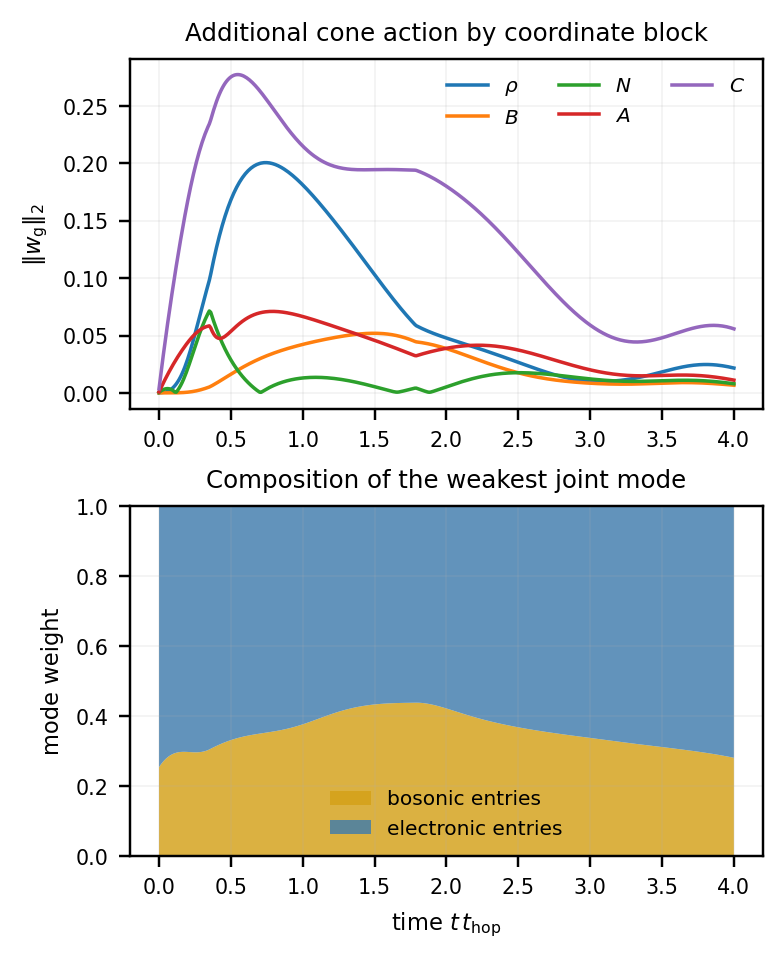
\includegraphics[width=0.82\linewidth]{MATH/paper_facing/paper_V_high_u_gkba/pedagogical/figures/joint_electron_phonon_mechanism_evidence.png}
        \caption{Correction mechanism. Upper: the part of \(w\) required by joint-Gram positive semidefiniteness beyond the trace and energy equalities; its two largest coordinate-block contributions to the integrated squared norm are \(69.18\%\) \(C\) and \(23.37\%\) \(\rho\). Lower: the time-resolved composition of the normalized eigenvector associated with \(\lambda_{\min}(\mathcal G)\); its correction-weighted average is \(62.97\%\) electronic and \(37.03\%\) bosonic.}
        \label{fig:paper-v-mechanism}
    \end{minipage}
\end{figure}

\end{document}
